%%%%%%%%%%%%
%
% $Autor: Zarzycki $
% $Datum: 2025-09-26 11:30:00Z $
% $Pfad: TemplateSensor $
% $Version: 4250 $
% !TeX spellcheck = en_GB/de_DE
% !TeX encoding = utf8
% !TeX root = filename 
% !TeX TXS-program:bibliography = txs:///biber
%
%%%%%%%%%%%%


% Structure
\chapter{Stromsensor SCT013-010}
	Dieses Kapitel behandelt Aufbau, Eigenschaften und praktische Anwendung des Stromsensors SCT013-010. Es beschreibt das Messprinzip des Stromwandlers, die elektrische Charakteristik sowie die Linearität des Sensors und erläutert die Bedeutung von Effektivwerten im Kontext der Wechselstrommessung. Zudem werden Schaltungsaufbau, Offset-Erzeugung, Tiefpassfilterung und die vollständige Verdrahtung mit dem Arduino MKR WAN 1310 dargestellt. Abschlie{\ss}end folgen Kalibrierungshinweise, Bibliotheksunterstützung und objektorientierte Codebeispiele zur Integration des Sensors in das Gesamtsystem.
	
\section{Allgemeines}
	Stromzangen ermöglichen die berührungslose Messung elektrischer Wechselströme, ohne den Leiter auftrennen oder den Stromkreis unterbrechen zu müssen \cite[2]{Lai:2025}. Dadurch eignen sie sich besonders für Anwendungen, bei denen eine einfache und sichere Installation wichtig ist, etwa bei der Energieverbrauchserfassung \cite{Najmurrokhman:2023}, der Überwachung elektrischer Systeme \cite{Lai:2025}, Fehlerdiagnose in industriellen Anwendungen\cite{Dhomad:2020}, \cite{Katsigiannis:2023} sowie der Fehlerdiagnose in Verteilnetzen \cite{Salum:2025}.
	


\section{Stromsensor SCT013-010}
	Der Stromsensor SCT013-010 zeichnet sich durch seine einfache Handhabung, hohe Genauigkeit, geringen Linearitätsfehler, niedrige Kosten sowie die Kompatibilität mit gängigen Mikrocontrollern aus \cite{Katsigiannis:2023}, \cite{YHDC:2017}. Er arbeitet nach dem Prinzip eines kleinen Transformators und liefert in der Regel eine Ausgangsspannung im Bereich von etwa $\pm 1\,\text{V}$ RMS (siehe~\autoref{sct:RMS}), die proportional zur Stromstärke (max. 10\,A RMS) ist \cite{Miron:2016}. Ein wesentlicher Vorteil des Sensors ist die galvanische Trennung zwischen dem zu messenden Leiter und dem Ausgangssignal \cite[480]{Meier:2022}. Dadurch bleibt das Messsystem zuverlässig von den höheren Netzspannungen isoliert und die Betriebssicherheit wird erheblich erhöht.

	
	
	
	\begin{figure}[H]
		\centering
		\begin{tikzpicture}
			\sctGeneral{0.5}{90}{0}{0}
			\draw[black, line width=0.35cm] (SCT-WIRE) -- ++(0.5,0) -- ++(0, -3.5) -- ++(-4, 0) coordinate (A);
			\draw[black, line width=0.15cm] ($(A) + (0, 0.1)$) -- ++(-0.5, 0) -- ++(0, 0.5) -- ++(-1, 0);
			\draw[red, line width=0.15cm] ($(A) + (0, -0.1)$) -- ++(-0.5, 0) -- ++(0, -0.5) -- ++(-1, 0);
		\end{tikzpicture}
		\caption{Stromsensor SCT013}
		\label{fig:sctGeneral}
	\end{figure}
	

\section{Funktionsprinzip \label{sctFunctionPrinciple}}
	Der SCT013-010 ist ein Stromwandler und arbeitet nach dem Prinzip eines kleinen Transformators (siehe~\autoref{fig:sctPrinciple}). Der durch die Primärleitung flie{\ss}ende Strom bildet die einwindige Primärwicklung, während auf der Gegenseite des Ferritkerns eine Sekundärwicklung mit vielen Windungen angebracht ist. Nach dem Ampèreschen Gesetz ist ein stromdurchflossener Leiter von einem Magnetfeld umgeben. Dieses Feld wird im Ferritkern des SCT013-010 gebündelt und durch das Sekundärwickel geführt. Da es sich beim Primärstrom um Wechselstrom handelt, verändert sich der magnetische Fluss zeitlich, wodurch gemä{\ss} dem Induktionsgesetz von Faraday im Sekundärwickel ein proportionaler Strom induziert wird. Dieser wird über den Burden-Widerstand in eine messbare Spannung umgesetzt. Im Fall des SCT013-010 dient die in die Klemme eingelegte Leitung als Primärwicklung. Der Ferritkern ist geteilt und befindet sich in Basis und Klemme, sodass ein Kabel mittig platziert werden kann. Am Sekundärausgang liegt eine Spannung von bis zu $\pm 1\,\text{V}$ RMS an, die von einem Mikrocontroller erfasst werden kann. Man muss aber sicherstellen, dass der durch diesen Sensor durchflossene Strom nicht $\pm 10\,A$ RMS überschreitet.

	Das Verhältnis der Ströme auf Primär- und Sekundärseite lässt sich durch folgende Gleichung beschreiben:
	\begin{equation}
		\frac{I_p}{I_s} = \frac{N_s}{N_p}
	\end{equation}
	wobei $I$ den Strom und $N$ die Anzahl der Windungen bezeichnet. Der Zusammenhang zwischen Sekundärstrom und Ausgangsspannung ergibt sich anschlie{\ss}end aus
	\begin{equation}
		U_s = I_s \cdot R_\text{Burden}.
	\end{equation}
	
	\begin{figure}[H]
		\centering
		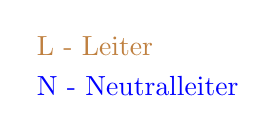
\begin{tikzpicture}
			\workingPrinciple{1}{0}{0}{0}
			
			\node [brown, anchor=west] at (-6, -5) {L - Leiter};
			\node [blue, anchor=west] at (-6, -5.5) {N - Neutralleiter};
		\end{tikzpicture}
		\caption{Prinzipieller Aufbau eines Stromsensors SCT013 \cite[480]{Meier:2022}}
		\label{fig:sctPrinciple}
	\end{figure}
	
	Der Stromsensor SCT013-010 verfügt über einen internen Burden-Widerstand, der eine Spannung am Ausgang von bis zu $\pm 1\,{V}$ RMS liefert.
	
	
	Die \autoref{fig:sct013-sinus-dualaxis} zeigt den Zusammenhang zwischen dem Strom auf der Primärseite und der Ausgangsspannung auf der Sekundärseite. Da es sich um Wechselstrom handelt, ändert sich dessen Richtung periodisch mit der Zeit. Dadurch ändert sich auch die Richtung des durch den Leiter erzeugten Magnetfeldes und dementsprechend das Potential der in der Sekundärwicklung induzierten Spannung. Somit ergibt sich bei einem Primärstrom von $\pm 10\,\text{A}$ RMS eine Ausgangsspannung von $\pm 1\,\text{V}$ RMS mit der Netzfrequenz von 50\,Hz (in Europa). Die Amplitude der Ausgangsspannung ist proportional zum gemessenen Strom (d.\,h. $\pm 5\,\text{A}$ RMS entsprechen $\pm 0{,}5\,\text{V}$ RMS auf der Sekundärseite (siehe \autoref{sctLinearity})).
	
	\begin{figure}[H]
		\centering
		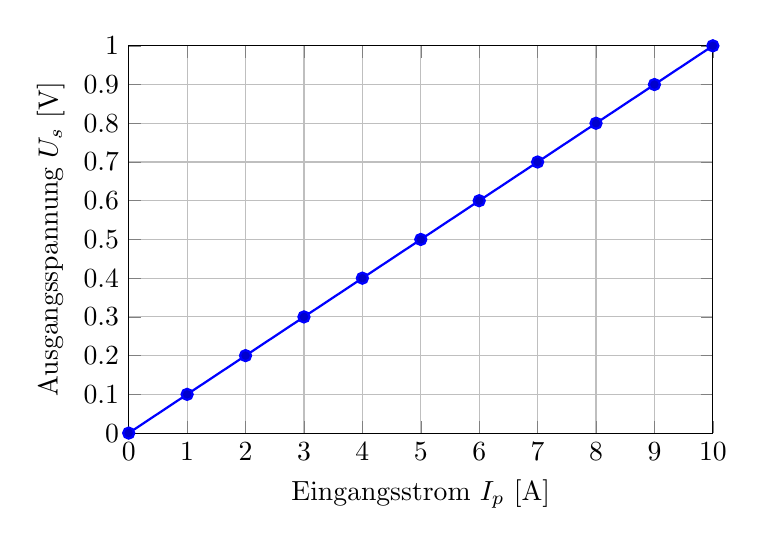
\begin{tikzpicture}
			\begin{axis}[
				width=9cm,
				height=6.5cm,
				grid=both,
				xlabel={Eingangsstrom $I_p$ [A]},
				ylabel={Ausgangsspannung $U_{s}$ [V]},
				xmin=0, xmax=10,
				ymin=0, ymax=1,
				xtick={0,...,10},
				ytick={0, 0.1,...,1},
				]
				% Messpunkte (abgelesen aus der Grafik)
				\addplot+[thick, blue, mark=*, smooth] coordinates {
					(0,0) (1,0.1) (2,0.2) (3,0.3) (4,0.4) (5,0.5)
					(6,0.6) (7, 0.7) (8, 0.8) (9, 0.9) (10, 1)
				};
			\end{axis}
		\end{tikzpicture}
		\caption{Zusammenhang zwischen Primärstrom und Ausgangsspannung \cite{YHDC:2017}}
		\label{fig:sct013-sinus-dualaxis}
	\end{figure}
	
\section{Effektivwert \label{sct:RMS}}
Der Effektivwert (RMS) bezeichnet diejenige Grö{\ss}e eines Wechselstroms oder einer Wechselspannung, die im Mittel die gleiche Leistung in einem ohmschen Widerstand erzeugt wie ein gleich gro{\ss}er Gleichstrom bzw. eine Gleichspannung \cite[255]{Stiny:2024}. 


\subsection{Berechnung des Effektivwertes}
	Der Effektivwert für sinusförmige Wechselgrö{\ss}en wird allgemein als Integral definiert:
	\begin{equation}
		U_\text{RMS} = \sqrt{\frac{1}{T} \int_0^T u^2(t)\,dt}.
	\end{equation}
	wobei $T = 2t$ (siehe~\autoref{fig:netzspannung}).
	
	Für eine Sinusspannung gilt:
	\begin{equation}
		u(t) = U_\text{peak} \cdot \sin(\omega t).
	\end{equation}
	
	Eingesetzt in die Definition:
	\begin{equation}
		U_\text{RMS} = \sqrt{\frac{1}{T} \int_0^T U_\text{peak}^2 \sin(\omega t)^2\,dt}.
	\end{equation}
	
	Mit der Identität 
	\[
	\sin(\omega t)^2 = \tfrac{1}{2}\left(1 - \cos(2\omega t)\right)
	\]
	vereinfacht sich das Integral zu:
	\begin{equation}
		\frac{1}{T}\int_0^T \sin(\omega t)^2\,dt 
		= \frac{1}{T}\int_0^T \frac{1}{2}\left(1 - \cos(2\omega t)\right)dt 
		= \frac{1}{2}.
	\end{equation}
	
	Damit folgt:
	\begin{equation}
		U_\text{RMS} = U_\text{peak} \cdot \sqrt{\tfrac{1}{2}} = \frac{U_\text{peak}}{\sqrt{2}}.
	\end{equation}
	
	Für die Netzspannung mit $U_\text{peak}=325$ V ergibt sich somit $U_\text{RMS}=230$ V.

	
	Das gleiche Vorgehen gilt auch für den Strom. Setzt man in die Definition den zeitabhängigen Verlauf 
	\begin{equation}
		i(t) = I_\text{peak} \cdot \sin(\omega t)
	\end{equation}
	ein, so ergibt sich in Analogie zur Spannung:
	\begin{equation}
		I_\text{RMS} = \frac{I_\text{peak}}{\sqrt{2}}.
	\end{equation}
	
	Für einen Spitzenwert von $I_\text{peak} = 14{,}1\,A$ ergibt sich somit ein Effektivwert von $I_\text{RMS} = 10\,A$ \cite[255--256]{Stiny:2024}
	
\subsection{Zusammenfassung der Spannungs- und Stromgrö{\ss}en}
	\begin{table}[H]
		\centering
		\begin{tabular}{|l|l|l|}
			\hline
			\textbf{Grö{\ss}e} & \textbf{Formel} & \textbf{Beispielwert} \\
			\hline
			Spitzenspannung & $U_\text{peak}$ & $325\,V$ \\
			Spitz-zu-Spitz-Spannung & $U_\text{pp} = 2U_\text{peak}$ & $650\,V$ \\
			Effektivwert & $U_\text{RMS} = \tfrac{U_\text{peak}}{\sqrt{2}}$ & $230\,V$ \\
			\hline
			Spitzenstrom & $I_\text{peak}$ & $14{,}1\,A$ \\
			Spitz-zu-Spitz-Strom & $I_\text{pp} = 2I_\text{peak}$ & $28{,}2\,A$ \\
			Effektivwert & $I_\text{RMS} = \tfrac{I_\text{peak}}{\sqrt{2}}$ & $10\,A$ \\
			\hline
		\end{tabular}
		\caption{Übersicht der verwendeten Spannungs- und Stromgrö{\ss}en}
		\label{tab:uebersicht-groessen}
	\end{table}
	
\subsection{Sinusförmige Beispiele und zugehörige Effektivwerte}
	Die folgenden Diagramme veranschaulichen den sinusförmigen Verlauf von Spannung und Strom sowie deren jeweilige Effektivwerte.
	
	\subsubsection{Beispiel: Netzspannung}
	
	% ============= Voltage 230  ==============
	\begin{figure}[H]
		\centering
		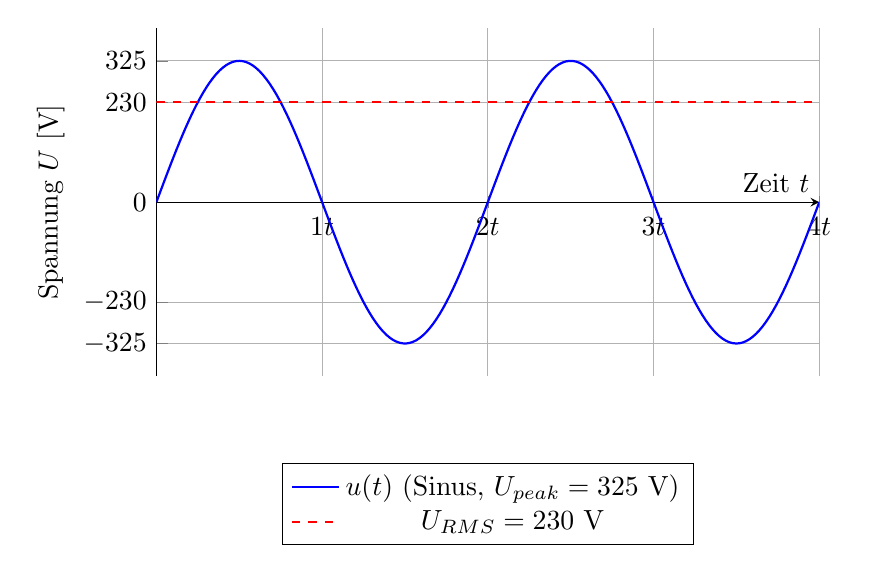
\begin{tikzpicture}
			\begin{axis}[
				width=10cm,
				height=6cm,
				axis y line*=left,
				axis x line=middle,
				xlabel={Zeit $t$},
				ylabel={Spannung $U$ [V]},
				xmin=0, xmax=40,
				ymin=-400, ymax=400,
				xtick={0,10,20,30,40},
				xticklabels={$0$, $1t$, $2t$, $3t$, $4t$},
				ytick={-325,-230,0,230,325},
				grid=both,
				major grid style={gray!60},
				minor grid style={gray!25},
				domain=0:40,
				samples=200,
				legend style={at={(0.5,-0.25)},anchor=north}
				]
				% sinus 325 V peak
				\addplot[blue, thick] {325*sin(deg(2*pi*50*x/1000))};
				\addlegendentry{$u(t)$ (Sinus, $U_{peak}=325$ V)}
				
				% RMS-Linie
				\addplot[dashed, red, thick] coordinates {(0,230) (40,230)};
				\addlegendentry{$U_{RMS} = 230$ V}
			\end{axis}
		\end{tikzpicture}
		\caption{Sinusförmige Netzspannung: $U_{RMS}=230$ V, $U_{peak}=325$ V, $U_{pp}=650$ V}
		\label{fig:netzspannung}
	\end{figure}
	
	\begin{align}
		U_\text{RMS} &= 230\,V \\
		U_\text{peak} &= U_\text{RMS} \cdot \sqrt{2} = 230 \cdot \sqrt{2} \approx 325\,V \\
		U_\text{pp} &= 2 \cdot U_\text{peak} \approx 650\,V
	\end{align}
	
	\subsubsection{Beispiel: Ausgang des Stromsensors SCT013-010}
		% ============= Voltage 1  ==============
	\begin{figure}[H]
		\centering
		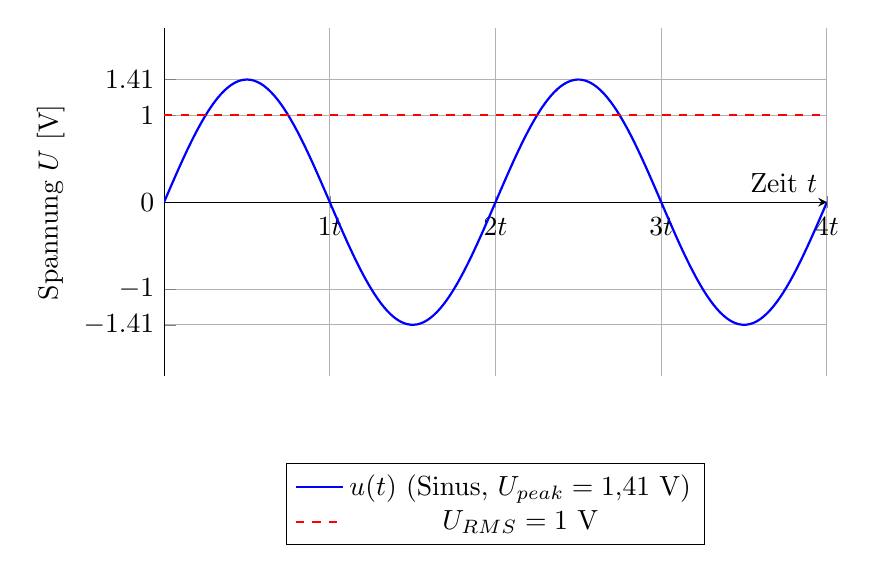
\begin{tikzpicture}
			\begin{axis}[
				width=10cm,
				height=6cm,
				axis y line*=left,
				axis x line=middle,
				xlabel={Zeit $t$},
				ylabel={Spannung $U$ [V]},
				xmin=0, xmax=40,
				ymin=-2, ymax=2,
				xtick={0,10,20,30,40},
				xticklabels={$0$, $1t$, $2t$, $3t$, $4t$},
				ytick={-1.41,-1,0,1,1.41},
				grid=both,
				major grid style={gray!60},
				minor grid style={gray!25},
				domain=0:40,
				samples=200,
				legend style={at={(0.5,-0.25)},anchor=north}
				]
				% sinus 1.41 V peak
				\addplot[blue, thick] {1.41*sin(deg(2*pi*50*x/1000))};
				\addlegendentry{$u(t)$ (Sinus, $U_{peak}=1{,}41$ V)}
				
				% RMS-Linien
				\addplot[dashed, red, thick] coordinates {(0,1) (40,1)};
				\addlegendentry{$U_{RMS} = 1$ V}
			\end{axis}
		\end{tikzpicture}
		\caption{Sinusförmige Ausgangsspannung des SCT013-010 für Eingangsstrom $10\,\text{A}$: $U_{RMS}=1\,\text{V}$, $U_{peak}=1{,}41\,\text{A}$, $U_{pp}=2{,}82\,\text{V}$}
		\label{fig:sct013-rms}
	\end{figure}
	
	Die Zusammenhänge lauten:
	\begin{align}
		U_\text{RMS} &= 1\,V \\
		U_\text{peak} &= U_\text{RMS} \cdot \sqrt{2} = 1 \cdot \sqrt{2} \approx 1{,}41\,V \\
		U_\text{pp} &= 2 \cdot U_\text{peak} \approx 2{,}82\,V
	\end{align}
	
	\subsubsection{Beispiel: Strom von 10 A (RMS)}

	% ============= Current ==============
	\begin{figure}[H]
		\centering
		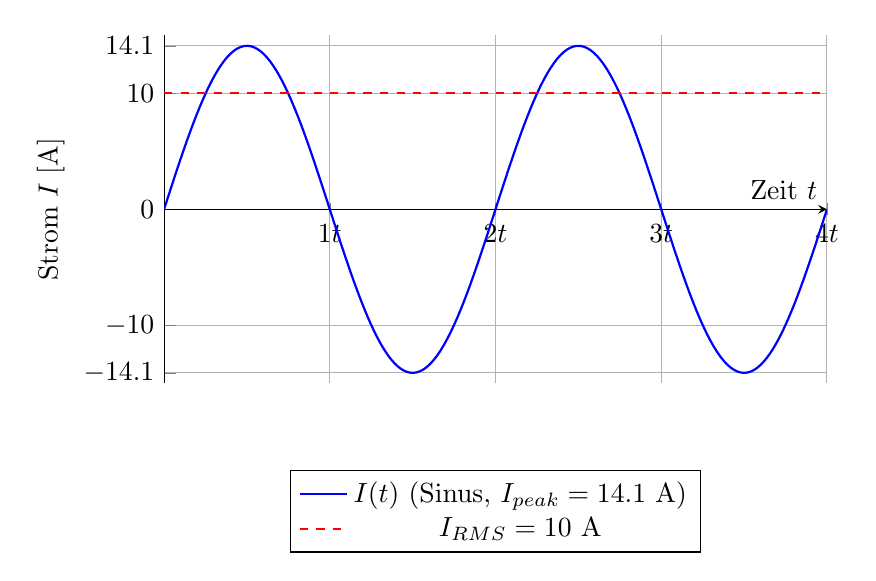
\begin{tikzpicture}
			% Linke Achse: RMS-Wert
			\begin{axis}[
				width=10cm,
				height=6cm,
				axis y line*=left,
				axis x line=middle,
				xlabel={Zeit $t$},
				ylabel={Strom $I$ [A]},
				xmin=0, xmax=40,
				ymin=-15, ymax=15,
				xtick={0,10,20,30,40},
				xticklabels={$0$, $1t$, $2t$, $3t$, $4t$},
				ytick={-14.1,-10,0,10,14.1},
				grid=both,
				major grid style={gray!60},
				minor grid style={gray!25},
				legend style={at={(0.5,-0.25)},anchor=north},
				domain=0:40,
				samples=200
				]
				% sinus 14.1 A peak
				\addplot[blue, thick] {14.1*sin(deg(2*pi*50*x/1000))};
				\addlegendentry{$I(t)$ (Sinus, $I_{peak}=14.1$ A)}
				
				% RMS-Linien
				\addplot[dashed, red, thick] coordinates {(0,10) (40,10)};
				\addlegendentry{$I_{RMS} = 10$ A}
			\end{axis}
		\end{tikzpicture}
		\caption{Sinusförmiger Strom: $I_{RMS}=10\,\text{A}$, $I_{peak}=14.1\,\text{A}$, $I_{pp}=28.2\,\text{A}$}
		\label{fig:strom-rms}
	\end{figure}
		
	\begin{align}
		I_\text{RMS} &= 10\,\text{A} \\
		I_\text{peak} &= I_\text{RMS} \cdot \sqrt{2} = 10 \cdot \sqrt{2} \approx 14{,}1\,\text{A} \\
		I_\text{pp} &= 2 \cdot I_\text{peak} \approx 28{,}2\,\text{A}
	\end{align}

	
	
% Voltage erstellung
\section{Linearität des Sensors \label{sctLinearity}}
	\textcite{Stiny:2024} definieren Linearität wie folgt:
	\begin{equation}
		Wirkung (n \cdot Ursache) = n \cdot Wirkung (\text{Ursache})
	\end{equation}
	In Worten: Die Wirkung der $n$-fachen Ursache entspricht der $n$-fachen Wirkung der einfachen Ursache. Dies verdeutlicht, dass Eingangs- und Ausgangsgrö{\ss}e in einem linearen Zusammenhang stehen.
	
	Im Fall eines Transformators gilt im Idealfall ein linearer Zusammenhang, sodass eine Verdopplung des Eingangsstroms auf der Primärseite auch zu einer Verdopplung des Ausgangsstroms auf der Sekundärseite führt \cite[480--484]{Meier:2022}. Abweichungen von dieser idealen Kennlinie werden als Linearitätsfehler bezeichnet. Der SCT013-010 weist mit einem Wert von höchstens 0,2\,\% (siehe \autoref{fig:sct013-characteristic}) einen geringen Linearitätsfehler auf \cite{YHDC:2017}. Dadurch genügt in der Praxis eine einfache Kalibrierung mit einem einzigen Faktor, um zuverlässige Messergebnisse über den gesamten Messbereich zu gewährleisten \cite{Earl:2024}. Im Folgenden wird, sofern nicht anders angegeben, bei allen Spannungs- und Stromgrö{\ss}en der Effektivwert (RMS) verwendet.

	
	\begin{figure}[H]
		\centering
		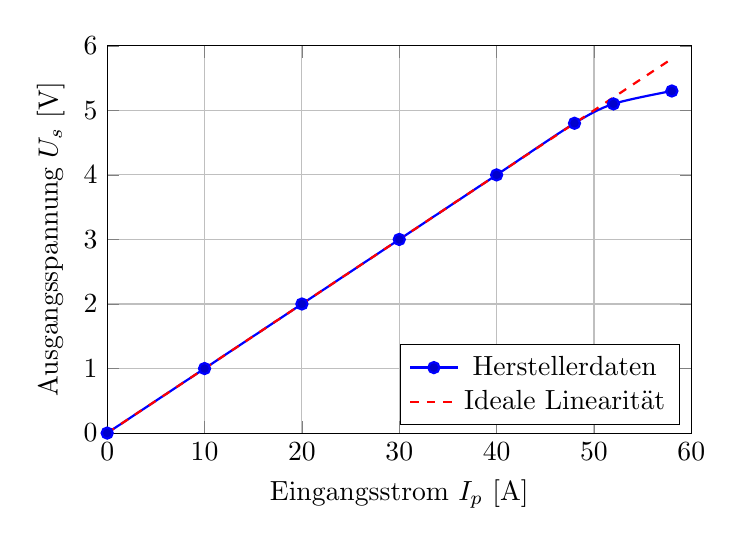
\begin{tikzpicture}
			\begin{axis}[
				width=9cm,
				height=6.5cm,
				grid=both,
				xlabel={Eingangsstrom $I_p$ [A]},
				ylabel={Ausgangsspannung $U_{s}$ [V]},
				xmin=0, xmax=60,
				ymin=0, ymax=6,
				xtick={0,10,20,30,40,50,60},
				ytick={0,1,2,3,4,5,6},
				legend style={at={(0.98,0.02)},anchor=south east}
				]
				% Messpunkte (abgelesen aus der Grafik)
				\addplot+[thick, blue, mark=*, smooth] coordinates {
					(0,0) (10,1) (20,2) (30,3) (40,4) (48,4.8)
					(52,5.1) (58,5.3)
				};
				\addlegendentry{Herstellerdaten}
				
				% Ideale Gerade (10 A = 1 V)
				\addplot[thick, red, dashed, domain=0:58] {x/10};
				\addlegendentry{Ideale Linearität}
			\end{axis}
		\end{tikzpicture}
		\caption{Kennlinie des SCT013-10\,A RMS /1\,V RMS laut Herstellerangaben \cite{YHDC:2017}}
		\label{fig:sct013-characteristic}
	\end{figure}

\section{Positive und negative Ausgangsspannung des Sensors \label{sctPosandNegOutputVoltage}}
Der wechselnde Eingangsstrom führt zu einer wechselnden Ausgangsspitzespannung im Bereich von $-1,41\,V$ bis $+1,41\,V$ (siehe~\autoref{fig:sct013-out}). 
Allerdings kann der \ac{adc} eines Mikrocontrollers meistens keine negativen Spannungen erfassen \cite{STMicro:2007}. 
Daher muss ein Bias angewendet werden, der die Spannung in den für den \ac{adc} nutzbaren Bereich verschiebt (siehe~\autoref{fig:sct013-out-bias}). 
Die Referenzspannung des Arduino MKR WAN 1310 beträgt 3,3\,V, weshalb sein \ac{adc} im Bereich von 0 bis 3,3\,V arbeitet \cite{Arduino:2020}. 
\autoref{fig:sct013-bias-circuit} zeigt ein Beispiel für Spannungsteilerschaltung, die den Bias auf 1,65\,V setzt, also genau die Hälfte der Referenzspannung des Arduino.



% --- Fig. 1: Ausgangsspannung ohne Offset ---
\begin{figure}[H]
	\centering
	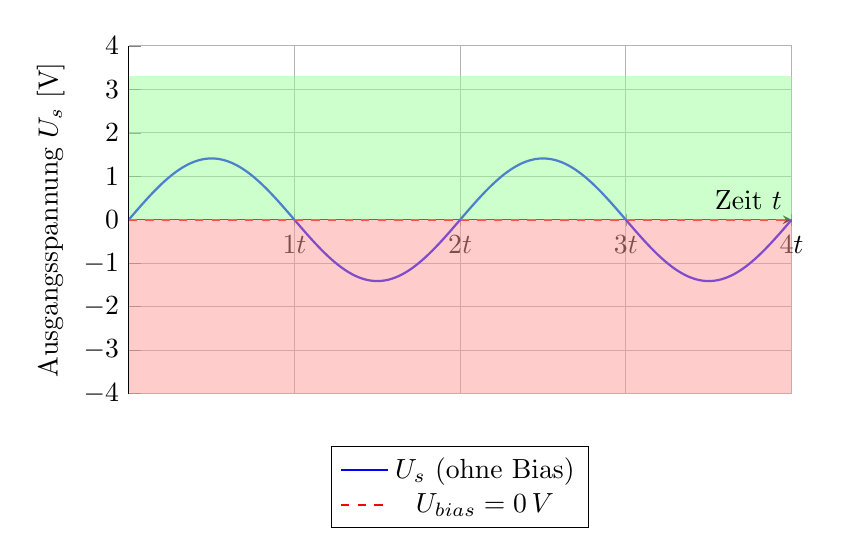
\begin{tikzpicture}
		\pgfplotsset{set layers}
		\begin{axis}[
			width=10cm,
			height=6cm,
			axis y line*=left,
			axis x line=middle,
			xlabel={Zeit $t$},
			ylabel={Ausgangsspannung $U_s$ [V]},
			xmin=0, xmax=40,
			ymin=-4, ymax=4,
			xtick={0,10,20,30,40},
			xticklabels={$0$, $1t$, $2t$, $3t$, $4t$},
			ytick={-4,..., 3.3, 4},
			grid=both,
			major grid style={gray!60},
			minor grid style={gray!25},
			legend style={at={(0.5,-0.15)},anchor=north},
			domain=0:40,
			samples=200
			]
			
			\addplot[blue, thick] {1.41*sin(deg(2*pi*50*x/1000))};
			\addlegendentry{$U_s$ (ohne Bias)}
			
			\addplot[dashed, red, thick] coordinates {(0,0) (40,0)};
			\addlegendentry{$U_{bias} = 0\,V$}
			
			\fill[green!40, opacity=0.5] (axis cs:0,0) rectangle (axis cs:40,3.3);
			\fill[red!40, opacity=0.5] (axis cs:0,0) rectangle (axis cs:40,-4);
		\end{axis}
	\end{tikzpicture}
	\caption{Ausgangsspannung $U_s$ des SCT013-10\,A/1\,V ohne Bias}
	\label{fig:sct013-out}
\end{figure}

% --- Fig. 2: Ausgangsspannung mit Offset ---
\begin{figure}[H]
	\centering
	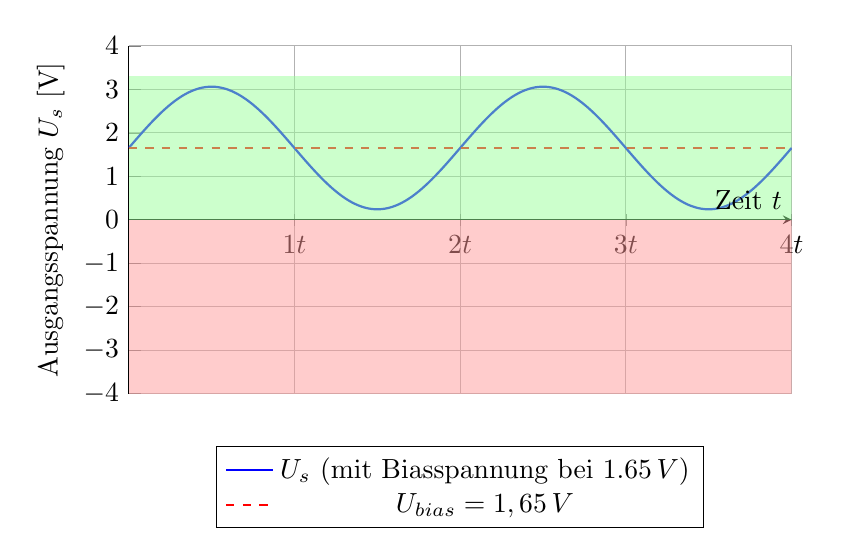
\begin{tikzpicture}
		\pgfplotsset{set layers}
		\begin{axis}[
			width=10cm,
			height=6cm,
			axis y line*=left,
			axis x line=middle,
			xlabel={Zeit $t$},
			ylabel={Ausgangsspannung $U_s$ [V]},
			xmin=0, xmax=40,
			ymin=-4, ymax=4,
			xtick={0,10,20,30,40},
			xticklabels={$0$, $1t$, $2t$, $3t$, $4t$},
			ytick={-4,..., 3.3, 4},
			grid=both,
			major grid style={gray!60},
			minor grid style={gray!25},
			legend style={at={(0.5,-0.15)},anchor=north},
			domain=0:40,
			samples=200
			]
			
			\addplot[blue, thick] {1.41*sin(deg(2*pi*50*x/1000))+1.65};
			\addlegendentry{$U_s$ (mit Biasspannung bei $1.65\,\text{V}$)}
			
			\addplot[dashed, red, thick] coordinates {(0,1.65) (40,1.65)};
			\addlegendentry{$U_{bias} = 1,65\,V$}
			
			\fill[green!40, opacity=0.5] (axis cs:0,0) rectangle (axis cs:40,3.3);
			\fill[red!40, opacity=0.5] (axis cs:0,0) rectangle (axis cs:40,-4);
		\end{axis}
	\end{tikzpicture}
	\caption{Ausgangsspannung $U_s$ des SCT013-10\,A/1\,V mit Offset in den ADC-Bereich von 0 - 3,3\,V verschoben}
	\label{fig:sct013-out-bias}
\end{figure}

% --- Fig. 3: Spannungsteiler ---
\subsection{Spannungsteiler zur Erzeugung Biasspannung}
	\begin{figure}[H]
		\centering
		\begin{circuitikz}[european]
			\draw(0,5) node[ocirc, label=left:\(VIN_{Arduino}\)]{} -- (3, 5)
			to[R, l_=$R_{10k}$, v^=$U_1$, i>_=$I_1$] (3, 2.5)
			to[R, l_=$R_{10k}$, *-*, v^=$U_2$, i>_=$I_2$] (3, 0) -- (0,0) node[ocirc, label=left:GND]{};
			\draw (3,2.5) -- ++(1.5,0) node[ocirc]{} node[right=2mm]{$VIN_{SCT013}$};
			\draw (3,0) -- ++(1.5,0) node[ocirc]{};
			\draw (4.5,2.5) to[open, v^=$U_{bias}$, voltage=straight, voltage shift=2] (4.5,0);
		\end{circuitikz}
		\caption{Widerstands-Spannungsteiler zur Erzeugung der Biasspannung $U_{bias}$ für den SCT013}
		\label{fig:sct013-bias-circuit}
	\end{figure}
	
	Die Wahl der Widerstände ($10,\text{k}\Omega$) und des Kondensators ($10,\mu\text{F}$) orientiert sich an der im OpenEnergyMonitor-Projekt vorgeschlagenen Schaltung \cite{OpenEnergyMonitor:2025}.

\subsubsection*{Berechnung des Offsets}
	Da der Spannungsteiler aus zwei gleichen Widerständen $R_1 = R_2 = 10\,\text{k}\Omega$ besteht, ergibt sich die Ausgangsspannung zu
	\begin{equation}
		U_{\text{bias}} = U_{\text{VCC}} \cdot \frac{R_2}{R_1 + R_2} 
		= 3{,}3\,\text{V} \cdot \frac{10}{20} = 1{,}65\,\text{V}.
	\end{equation}
	Damit liegt der Offset exakt bei der Hälfte der Versorgungsspannung und bildet den Arbeitspunkt (Biasspannung) für das Sensorsignal \cite[91--92]{Meier:2022}.


\section{Tiefpassfilter zur Stabilisierung der Biasspannung}
	Wie im \autoref{sctPosandNegOutputVoltage} beschrieben, muss die Ausgangsspannung des SCT013 durch eine Biasspannung verschoben werden, damit der \ac{adc} des Arduino den vollständigen Spannungsverlauf erfassen kann. Da jedoch im Gesamtsystem des Arduino spontane Spannungsschwankungen oder andere langsame Fluktuationen auftreten können, ist eine zusätzliche Stabilisierung der Biasspannung erforderlich. Zu diesem Zweck wird zusammen mit Spannungsteiler (siehe~\autoref{fig:sct013-bias-circuit}) ein RC-Tiefpassfilter eingesetzt  (siehe~\autoref{fig:sct013-low-pass-filter}.
	
		
	\begin{figure}[H]
		\centering
		\begin{circuitikz}[european]
			\draw(0,5) node[ocirc, label=left:\(VIN_{Arduino}\)]{} -- (3, 5)
			to[R, l_=$R_{10k}$] (3, 2.5)
			to[R, l_=$R_{10k}$, *-*] (3, 0) -- (0,0) node[ocirc, label=left:GND]{};
			\draw (3,2.5) -- ++(1.5,0) node[ocirc]{} node[right=2mm]{$VIN_{SCT013}$};
			\draw (3,0) -- ++(1.5,0) node[ocirc]{};
			\draw (4.5,2.5) to[open, v^=$U_{bias}$, voltage=straight, voltage shift=2] (4.5,0);
			\draw (3,2.5) -- (1,2.5) to[C, l_=$10\,\mu\text{F}$, -*] (1,0);
			
		\end{circuitikz}
		\caption{Widerstands-Spannungsteiler mit Kapazitor zur Erzeugung des Biasspannung $U_{bias}$ für den SCT013}
		\label{fig:sct013-low-pass-filter}
	\end{figure}
	
	Ein RC-Tiefpassfilter überträgt niedrige Frequenzen nahezu unverändert, während hohe Frequenzanteile in ihrer Amplitude abgeschwächt werden \cite{Stiny:2024}. Im vorliegenden Anwendungsfall dient der Tiefpass nicht zur Filterung des Messsignals selbst, sondern zur Stabilisierung der Biasspannung. Dadurch wird verhindert, dass der Offsetpunkt (Biasspannung) unkontrolliert schwankt.
	
	Langsame Änderungen der Versorgungsspannung (z. B. ein allmähliches Ansteigen oder Abfallen der VCC-Pins) können durch den Kondensator nachgebildet werden: Er lädt bzw. entlädt sich entsprechend, sodass der Offset kontrolliert mitverschoben wird. Plötzliche Spannungssprünge hingegen werden vom Kondensator unterdrückt und nicht direkt an den Offsetpunkt weitergegeben. Auf diese Weise bleibt die Bezugsspannung stabil, und das Risiko verfälschter oder verstärkter Messwerte wird minimiert.

\subsection{Zeitkonstante}
	\textcite{Stiny:2024} beschreibt die Zeitkonstante (\tau) als ein Ma{\ss} dafür, wie schnell die Spannung am Kondensator ansteigt bzw. der Strom abfällt. Sie gibt an, nach welcher Zeit das Ansteigen der Spannung beziehungsweise das Abfallen der Stromstärke „nahezu abgeschlossen“ ist. Nach Ablauf einer Zeitkonstante hat die Spannung am Kondensator etwa 63\,\% der Ladespannung erreicht, während der Strom auf rund 37\,\% des Anfangswertes abgefallen ist.

\begin{equation}
	\tau = R \cdot C
\end{equation}

	Dabei ist $\tau$ die Zeitkonstante in Sekunden, $R$ der Widerstand in Ohm und $C$ die Kapazität in Farad.
	
	Nach einer weiteren Zeitspanne von $\tau$ steigt die Spannung von den verbleibenden 37\,\% erneut um 63\,\% an, sodass rund 86,3\,\% der Endspannung erreicht sind. Der Strom sinkt entsprechend auf etwa 13,7\,\% des Anfangswertes. Nach dem Ablauf von fünf Zeitkonstanten gilt der Kondensator praktisch als vollständig aufgeladen (ca. 99,3\,\%) \cite[174--176]{Stiny:2024}.
	
\subsubsection*{Berechnungsbeispiel}
	Für die in diesem Projekt verwendeten Werte $R = 10\,\text{k}\Omega$ und $C = 10\,\mu\text{F}$ ergibt sich eine Zeitkonstante von
	\begin{equation}
		\tau = R \cdot C = 10{,}000 \,\Omega \cdot 10 \times 10^{-6}\,\text{F} = 0{,}1 \,\text{s}.
	\end{equation}

	
\subsection{Grenzfrequenz}
	Die Grenzfrequenz ($f_g$) gibt an, ab welcher Frequenz ein RC-Tiefpassfilter das Eingangssignal zunehmend abschwächt. Per Definition ist die Amplitude bei der Grenzfrequenz bereits auf den Faktor 
	\(\tfrac{1}{\sqrt{2}} \approx 0{,}707\) des ursprünglichen Wertes abgesunken \cite[340]{Stiny:2024}.
	
	Die Grenzfrequenz berechnet sich zu
	\begin{equation}
		f_g = \frac{1}{2 \pi R C} = \frac{1}{2 \pi \cdot 0{,}1\,\text{s}} \approx 1{,}6 \,\text{Hz}.
	\end{equation}
	
	Damit liegt die Grenzfrequenz weit unterhalb der Netzfrequenz von 50\,Hz. Folglich bleibt das Nutzsignal des Stromsensors unbeeinträchtigt, während die Biasspannung stabilisiert wird.
	
	\subsubsection*{Zusammenhang mit der Zeitkonstante}
	Zwischen Zeitkonstante \(\tau\) und Grenzfrequenz \(f_c\) besteht folgender Zusammenhang:
	\[
	f_g =  \frac{1}{2 \pi R C} = \frac{1}{2 \pi \cdot 0{,}1\,\text{s}} = \frac{1}{2 \pi \tau}.
	\]
	
	Ein gro{\ss}es Produkt \(R \cdot C\) führt zu einer gro{\ss}en Zeitkonstante \(\tau\). Dadurch reagiert der Filter träge, und die Grenzfrequenz \(f_c\) wird sehr klein – der Filter lässt dann nur sehr langsame Änderungen passieren. Umgekehrt bewirkt ein kleines \(R \cdot C\) eine kurze Zeitkonstante und damit eine höhere Grenzfrequenz, sodass auch schnellere Signalanteile übertragen werden.
	
		
	
	
\section{Verkabelung mit Arduino MKR WAN 1310}
	Ausgehend von der in \autoref{fig:sct013-low-pass-filter} dargestellten Schaltung ergibt sich die in \autoref{fig:verkabelung-sct013} gezeigte Verdrahtung zwischen dem Stromsensor SCT013-010 und dem Arduino MKR WAN 1310. Der Stromsensor ist mit dem analogen Pin A0 des Arduinos verbunden.
	
	\begin{figure}[H]
		\centering
		\begin{tikzpicture}
			\ArduinoMkrWan{0.5}{-90}{0}{0}{0}
			\resistorTHT{0.3}{90}{-5}{3.8}{2}{A}
			\resistorTHT{0.3}{90}{-3.8}{3.8}{2}{B}
			\sctGeneral{0.3}{270}{3}{6}
			
			\draw[line width=0.1cm, red] (mkrPin-VCC) -- ++ (0, 0.75) -| (RES-LEFT-A);
			\draw[line width=0.1cm, black] (mkrPin-GND) -- ++ (0, 1) coordinate(A) -| (RES-LEFT-B);
			
			
			% Capacitor
			\node[coordinate] (Cap) at (-2.5, 3.8) {};
			\fill[black] (Cap) circle (0.7cm);
			\fill[gray!40] (Cap) circle (0.5cm);
			\node[black] at ($(Cap) + (0, 0.3)$) {\Large$\pmb{+}$};
			\node[black] at ($(Cap) + (0, -0.3)$) {\Large$\pmb{-}$};
			\draw[line width=0.1cm, gray] ($ (Cap) + (0,-0.7cm) $) -- (A -| Cap); 
			
			\draw[line width=0.1cm, Orange] (RES-RIGHT-A) -- ++(0, 0.5) -| ($ (Cap) + (0,0.7cm) $);
			
			% wires to SCT013
			\draw[line width=0.1cm, Orange] (RES-RIGHT-B) |- ($(SCT-WIRE)+(0, 0.05)$);
			\draw[line width=0.1cm, red] (mkrPin-A1) -- ++(0, -0.8) -- ++(6.3, 0) -- ++(0, 5) -| ($(SCT-WIRE)+(0, 0.0)$);
		\end{tikzpicture}
		\caption{Verdrahtung des SCT013-010 mit dem Arduino MKR WAN 1310}
		\label{fig:verkabelung-sct013}
		
	\end{figure}

\section{Anschluss an den Leiter}
	Es ist zu beachten, dass die Stromzange nicht um das gesamte Kabel, sondern ausschlie{\ss}lich um eine einzelne Leitung gelegt werden darf. Da der Wechselstrom gleichzeitig in Hin- und Rückleiter flie{\ss}t, würden sich die entgegengesetzt gerichteten Magnetfelder gegenseitig aufheben (siehe~\autoref{sctFunctionPrinciple}). Deshalb muss die Stromzange um die Leiterader \emph{L} (Phase) angeschlossen werden, sodass das resultierende Magnetfeld einer einzelnen Leitung erfasst werden kann.

	\begin{figure}[H]
		\centering
		\resizebox{0.7\textwidth}{!}{%
			\begin{tikzpicture}
				% SCT013
				\fill[blue] (-1,0) rectangle (1,4);
				\draw[black, line width=0.3cm](0,0) -- ++(0, -1);
				\draw[black, line width=0.05cm] (-1, 4) -- (-0.8, 2) -- (0.8, 2) -- (1, 4);
				\draw[black, line width=0.05cm] (-0.8, 2) -- (-0.8, 1.8) -- (0.8, 1.8) -- (0.8, 2);
				
				% 230V cable
				\draw[black, line width=1cm] (-6, 5) -- (-3,5) coordinate(A);
				\draw[black, line width=1cm] (6, 5) -- (3,5) coordinate (B);
				
				% single wires
				\draw[yellow, line width=0.3cm] ($(A) + (0, 0.35)$) -- ($(B) + (0, 0.35)$);
				\draw[blue, line width=0.3cm] ($(A) + (0, 0.0)$) -- ($(B) + (0, 0.0)$);
				\draw[brown, line width=0.3cm] ($(A) + (0, -0.35)$) -- ++(0.5, 0) |- (-1, 3);
				\draw[brown, line width=0.3cm] ($(B) + (0, -0.35)$) -- ++(-0.5, 0) |- (1, 3);
				
				\draw[red, line width=0.1cm, <-,  >=stealth] (-4.5, 5) -- ++(0.5, -3) node[below] {\Large{Kabel 230\,V}};
				\draw[red, line width=0.1cm, <-,  >=stealth] (4.5, 5) -- ++(-0.5, -3) node[below] {\Large{Kabel 230\,V}};
				\draw[red, line width=0.1cm, <-,  >=stealth] (0, 1) -- ++(0.5, -1.5) node[right] {\Large{Stromsensor SCT013-010}};
			\end{tikzpicture}%
		}
		\caption{Anschluss des SCT013-010 an eine einzelne Leiterader des Netzkabels}
		\label{fig:sct013-anschluss}
	\end{figure}
		



\section{Specification}
\subsection{Technische Daten}

\begin{table}[H]
	\centering
	\begin{tabular}{|l|l|}
		\hline
		\textbf{Parameter} & \textbf{Wert} \\
		\hline
		Nennstrom (rms) & 10 A \\
		\hline
		Maximalstrom & 35 A \\
		\hline
		Nennausgang & 1 V \\
		\hline
		Genauigkeit & $\pm$1 \% \\
		\hline
		Linearität & $\leq$0,2 \% \\
		\hline
		Gewicht & 50 g \\
		\hline
		Arbeitsspannung & 660 V \\
		\hline
		Frequenzbereich & 50 Hz – 1 kHz \\
		\hline
		Betriebstemperatur & -25 °C bis +70 °C \\
		\hline
		Lagertemperatur & -30 °C bis +90 °C \\
		\hline
		Isolationsfestigkeit & 3,5 kV (50 Hz, 1 min) \\
		\hline
	\end{tabular}
	\caption{Technische Daten des SCT013-010 Stromsensors \cite{YHDC:2017}}
	\label{tab:SCT013-Daten}
\end{table}


\section{Bibliotheken}
	\subsection{Bibliothek \PYTHON{EmonLib}}
	Die Bibliothek \PYTHON{EmonLib} ermöglicht die Messung von Strom, Spannung und Leistung in Echtzeit. Sie wurde im Rahmen des Projekts \textit{OpenEnergyMonitor} entwickelt und dient der Analyse von elektrischen Signalen in Niederspannungsschaltungen. Die Bibliothek verarbeitet analoge Eingangssignale von Strom- und Spannungssensoren, indem sie eine sogenannte \textit{Sampling}-Methode anwendet. Dabei werden viele Einzelmessungen innerhalb eines bestimmten Zeitraums erfasst und anschlie{\ss}end ausgewertet, um den effektiven Effektivwert von Strom und Spannung zu bestimmen. Die in der Bibliothek implementierten Algorithmen berücksichtigen den in der Schaltung vorhandenen Offset und entfernen diesen automatisch mithilfe eines digitalen Tiefpassfilters. 
	
	
	\subsubsection{Installation}
	Diese Bibliothek kann über die PlatformIO-Registry \cite{OpenEnergyMonitor:2014PIO} oder direkt über GitHub \cite{OpenEnergyMonitor:2014GIT} bezogen werden. In den folgenden Beispielen wird die Version 1.1.0 verwendet.
	
	Nach der Installation der Bibliothek und der Implementierung in der Datei \FILE{platformio.ini} muss die Header-Datei \FILE{EmonLib.h} in das Projekt eingebunden werden.


	\subsubsection{Funktionen}
		\begin{description}
		\item \PYTHON{EnergyMonitor emon;} \\ 
		Konstruktor für ein \PYTHON{EnergyMonitor} - Objekt.  Er erstellt eine neue Instanz der Klasse, die zur Erfassung und Berechnung des elektrischen Stromes dient. Beim Erstellen des Objekts werden noch keine Pins oder Kalibrierwerte definiert.
		
		
		\item \PYTHON{emon.current(pinI, calibVal)} \\ 
		Initialisiert den Eingang für den Stromsensor. 
		Der Parameter \PYTHON{pinI} legt den analogen Eingangspin fest, an dem der Sensor angeschlossen ist. 
		Der Parameter \PYTHON{calibVal} ist der Kalibrierungsfaktor, der den gemessenen Rohwert in Ampere umrechnet. 
		Dieser Wert muss an bestimmten Sensor angebasst werden, da er vom verwendeten Sensor und der Schaltung abhängt (siehe~\autoref{sct:calibration}).
		
		
		\item \PYTHON{emon1.calcIrms(Number\_of\_Samples)} \\ 
		 Führt eine Strommessung mit der angegebenen Anzahl von Messproben durch. Die Funktion ermittelt den Effektivwert des Stroms in Ampere, indem sie die Signale mehrfach abtastet, filtert und den Mittelwert der Quadrate berechnet. Der Rückgabewert ist die gemessene Stromstärke \textit{Irms} in Ampere und wird als \PYTHON{double} zurückgegeben.
		
	\end{description}
		
	\subsection{Kalibrierung des Stromsensors \label{sct:calibration}}
	
	Die Kalibrierung des Stromsensors basiert auf der Beziehung zwischen dem Primärstrom, der Übersetzung des Stromwandlers und dem Belastungswiderstand. 
	Ein Stromwandler (in diesem Fall der Stromsensor \textit{SCT-013}) erzeugt aus dem Primärstrom \(I_p\) einen kleineren Sekundärstrom \(I_s\), der über den Belastungswiderstand \(R_b\) in eine messbare Spannung \(U_s\) umgewandelt wird. 
	Das Verhältnis zwischen Primär- und Sekundärstrom wird durch die Übersetzung \(k = \frac{I_p}{I_s}\) beschrieben. 
	Die am ADC anliegende Spannung ergibt sich somit zu:
	\[
	U_s = I_s \cdot R_b = \frac{I_p}{k} \cdot R_b
	\]
	
	Diese Spannung wird anschlie{\ss}end durch den ADC in eine vom Prozessor messbare Grö{\ss}e umgewandelt:
	\[
	ADC_{val} = \frac{U_s}{U_{ref}} \cdot ADC_{max}
	\]
	
	Setzt man diese Gleichung in den vorherigen Zusammenhang ein, ergibt sich für den Primärstrom:
	\[
	I_p = \frac{ADC_{val}}{ADC_{max}} \cdot U_{ref} \cdot \frac{k}{R_b}
	\]
	
	Da der Ausdruck \(\frac{k}{R_b}\) die Umrechnung vom gemessenen Spannungssignal in den tatsächlichen Primärstrom beschreibt, wird er als sogenannte \textit{calibration constant} definiert:
	\[
	calibration\ constant = \frac{k}{R_b}
	\]
	
	Somit kann der Primärstrom vereinfacht berechnet werden als:
	\[
	I_p = \frac{ADC_{val}}{ADC_{max}} \cdot U_{ref} \cdot calibration\ constant
	\]
	
	Bei Sensoren mit eingebautem Belastungswiderstand (wie dem \textit{SCT-013-010}) vereinfacht sich die Berechnung, da der Hersteller direkt den Zusammenhang zwischen Ausgangsspannung und Primärstrom angibt:
	\[
	calibration\ constant = \frac{I_p}{U_s}
	\]
	
	Beispielsweise liefert der Sensor \textit{SCT-013-010} bei einem Primärstrom von 10\,A eine Ausgangsspannung von 1\,V. 
	Hier beträgt der Kalibrierungsfaktor:
	\[
	calibration\ constant = \frac{10}{1} = 10
	\]
	
	Aufgrund von Toleranzen in den Bauteilen und anderen Einflüssen können die gemessenen Werte leicht abweichen. 
	Daher sollte der theoretisch berechnete Kalibrierungswert überprüft und bei Bedarf so angepasst werden, 
	dass die Messergebnisse mit einer Referenzmessung (z.\,B. mit einem Multimeter) übereinstimmen bzw. innerhalb akzeptabler Toleranzen liegen \cite{OpenEnergyMonitor:2023}.
	
	
\section{Code Beispiele}
\subsection{Auslesen des Stromes}
	Das folgende Beispiel demonstriert die Verwendung der Bibliothek \PYTHON{EmonLib} zur Messung des elektrischen Stroms mithilfe des Stromsensors SCT-013-010. Das Sensorsignal wird über den analogen Eingang des Mikrocontrollers eingelesen. Die Funktion \PYTHON{current(currentPin, calibVal)} initialisiert dabei den Messkanal mit dem angegebenen Eingangspin \PYTHON{currentPin = A0} und mit einem Kalibrierungsfaktor \PYTHON{calibVal = 111.1}, der die Umrechnung zwischen dem analogen Messsignal und dem tatsächlichen Stromwert in Ampere ermöglicht. Zur Berechnung des Effektivwerts wird die Funktion \PYTHON{calcIrms(samplesAmount)} verwendet, die 1480 Messwerte (Samples) innerhalb eines kurzen Zeitintervalls erfasst und daraus den RMS-Wert des Stroms bestimmt. Der berechnete Effektivstrom repräsentiert den tatsächlichen Stromfluss im Stromkreis und wird im seriellen Monitor ausgegeben.
	
	
	{
		\captionof{code}{Effektivwert des elektrischen Stromes Auslesen}
		\ArduinoExternal{}{../../Code/MKRWAN1310/CurrentSensorSCT013/currentMeasurement.cpp}
	}
	
\subsection{Objektorientierte Strommessung}

	Im folgenden Beispiel wird gezeigt, wie die Strommessung mithilfe des Sensors SCT-013-010 objektorientiert umgesetzt werden kann. Hierzu wird die Bibliothek \PYTHON{EmonLib} in einer eigenen Klasse \PYTHON{CCurrentSensor} gekapselt, die eine saubere Trennung zwischen Hardwareansteuerung und Programmstruktur ermöglicht. 
	
	Die Klasse übernimmt die Initialisierung, die Kalibrierung sowie das Auslesen des Effektivwerts des Stroms. 
	Über die Methode \PYTHON{init()} wird der Sensor mit dem analogen Eingangspin (\PYTHON{A1}) und einem Kalibrierungsfaktor \PYTHON{10.1} konfiguriert, 
	der die Umrechnung des analogen Signals in den tatsächlichen Stromwert (Ampere) ermöglicht. 
	Die Methode \PYTHON{readCurrent(currentOut)} ruft intern die EmonLib-Funktion \PYTHON{calcIrms(samples)} auf, 
	wobei \PYTHON{samples = 1480} Einzelmessungen zur Berechnung des Effektivwerts herangezogen werden. 
	
	Das Ergebnis wird als Rückgabewert über eine Referenzvariable ausgegeben, während der Funktionsstatus (\PYTHON{CSError}) den Erfolg oder mögliche Fehler signalisiert. Alle Meldungen an den Benutzer werden über die Hilfsklasse \PYTHON{MessagesENG} im seriellen Monitor ausgegeben. 
	
	{
		\captionof{code}{Header-Datei der Nachrichtenverwaltung}
		\ArduinoExternal{}{../../Code/MKRWAN1310/CurrentSensorSCT013/Messages.h}
	}
	
	{
		\captionof{code}{Implementierung der Methoden der Nachrichtenverwaltung}
		\ArduinoExternal{}{../../Code/MKRWAN1310/CurrentSensorSCT013/Messages.cpp}
	}
	
	{
		\captionof{code}{Hilfsfunktionen für serielle Ein- und Ausgaben}
		\ArduinoExternal{}{../../Code/MKRWAN1310/CurrentSensorSCT013/SerialUtils.h}
	}
	
	{
		\captionof{code}{Implementierung der Funktionen für serielle Ein- und Ausgaben}
		\ArduinoExternal{}{../../Code/MKRWAN1310/CurrentSensorSCT013/SerialUtils.cpp}
	}
	
	{
		\captionof{code}{Header-Datei der Stromsensor-Klasse}
		\ArduinoExternal{}{../../Code/MKRWAN1310/CurrentSensorSCT013/CCurrentSensor.h}
	}
	
	{
		\captionof{code}{Implementierung der Methoden der Stromsensor-Klasse}
		\ArduinoExternal{}{../../Code/MKRWAN1310/CurrentSensorSCT013/CCurrentSensor.cpp}
	}
	
	{
		\captionof{code}{Beispielprogramm zur Verwendung der Stromsensor-Klasse}
		\ArduinoExternal{}{../../Code/MKRWAN1310/CurrentSensorSCT013/main.cpp}
	}

	
	

%\subsection{Description}

%\subsection{Installation}

%\subsection{Functions}

%\subsection{Example - Manual}

%\subsection{Example}

%\subsection{Example - Code}

%\subsection{Example - Files}






%\section{Simple Code}


%\section{Einfache Application}



%\section{Tests}

%\subsection{Simple Function Test}

%\subsection{Test all Functions}

%\section{Simple Application}


%\section{Further Readings}

